\chapter{Analysis of the wheelchair locomotion}

\section{Introduction}
Wheelchair locomotion concerns many people, for different reasons: genetic(myopathy), accidental (spinal cord injury, lower extremity amputee), degenerative (multiple sclerosis, poliomyelitis) or just related to the natural aging of locomotor functions (muscle degeneration, arthritis of the lower limbs, etc.). Then, in the 34 developed countries, it is estimated that 1\% or 10,000,000 people require a wheelchair. In the 156 developing countries, it is estimated that at least 2\% or 121,800,000 people require a wheelchair. Overall, of the 7,091,500,000 people in the world, approximately 131,800,000 or 1.85\% need a wheelchair [].%https://www.wheelchairfoundation.org/programs/from-the-heart-schools-program/materials-and-supplies/analysis-of-wheelchair-need/
However, the use of the manual wheelchair is not without risk.

\section{The problem of locomotion manual wheelchair locomotion}

Although the use of FRM improves the mobility of its users, doctors quickly realized that its use often led to sedentarization, leading to problems of obesity, diabetes, etc. Also, to promote daily physical activity, sport has been strongly encouraged [147, 203, 211, 259]. However, intensive and prolonged sports practice in FRM can lead to specific injuries and pains [79, 125, 274, 277], especially in the shoulder [11, 14, 25, 79, 192,], and at the elbow, wrist and hand [140, 141, 241, 232 279, 295, 352]. Thus, according to studies conducted between 1991 and 2000, it has been reported that 30 [11] to 73\% [241] of paraplegic individuals suffered from shoulder pain. In addition, sitting and prolonged sitting of FRM users causes dermatological problems such as bedsores or pressure ulcers, due to immobility, loss of sensitivity and incontinence. In addition, these symptoms are recognized as a major cause of discontinuation of the use of FRM [314, 336], thus the sedentarization of users. Lundqvist et al. [210] showed that upper limb pain was the only factor correlated with poor quality of life in FRM subjects. The difficulty for the therapist is to practice a daily physical activity, adapted to the individual, and limit orthopedic problems and thus promote the use of the FRM over time.


Given the problems faced by manual wheelchair users at the level of
their autonomy and health, van der Woude et al. [304, 305] summarized the issues of manual wheelchair locomotion research into three main areas:

\begin{itemize}
\item Improving the interface between the subject and his manual wheelchair, that is to say, the ergonomy and the adequacy of the system \{subject + manual wheelchair\} with the external physical environment (ramps, lifts, corridor widths, etc.).
\item The improvement of the manual wheelchair regarding the design and the mechanical principles of propulsions;
\item \textbf{Improving the subject's physical abilities}, that is, improving propulsion techniques, as well as rehabilitation techniques and training programs.
\end{itemize}

Bio-mechanics work has been conducted in LIMOS to identify and quantify traumatic factors such as. This work led to the construction of a measuring tool: an Ergo-meter Field Chair.

\section{Tools to evaluate manual wheelchair locomotion}

\section{Knowledge discovery on wheelchair time series}

Locomotion in manual wheelchair causes significant mechanical stresses in the upper limbs. To remedy this problem, biomechanics have been conducted to identify and quantify traumatic factors such as:
\begin{itemize}
\item The doctoral thesis of Nicolas de Saint REMY (2005) [1] who proposed a
mechanical model relating the forces applied to a Manual Wheelchair and its displacement as illustrated in Figure 1.1 and Equation 1.1. It made it possible to highlight the fact that the acceleration of the FRM is a function of the movements of the subject:

\begin{figure}[h]
\center
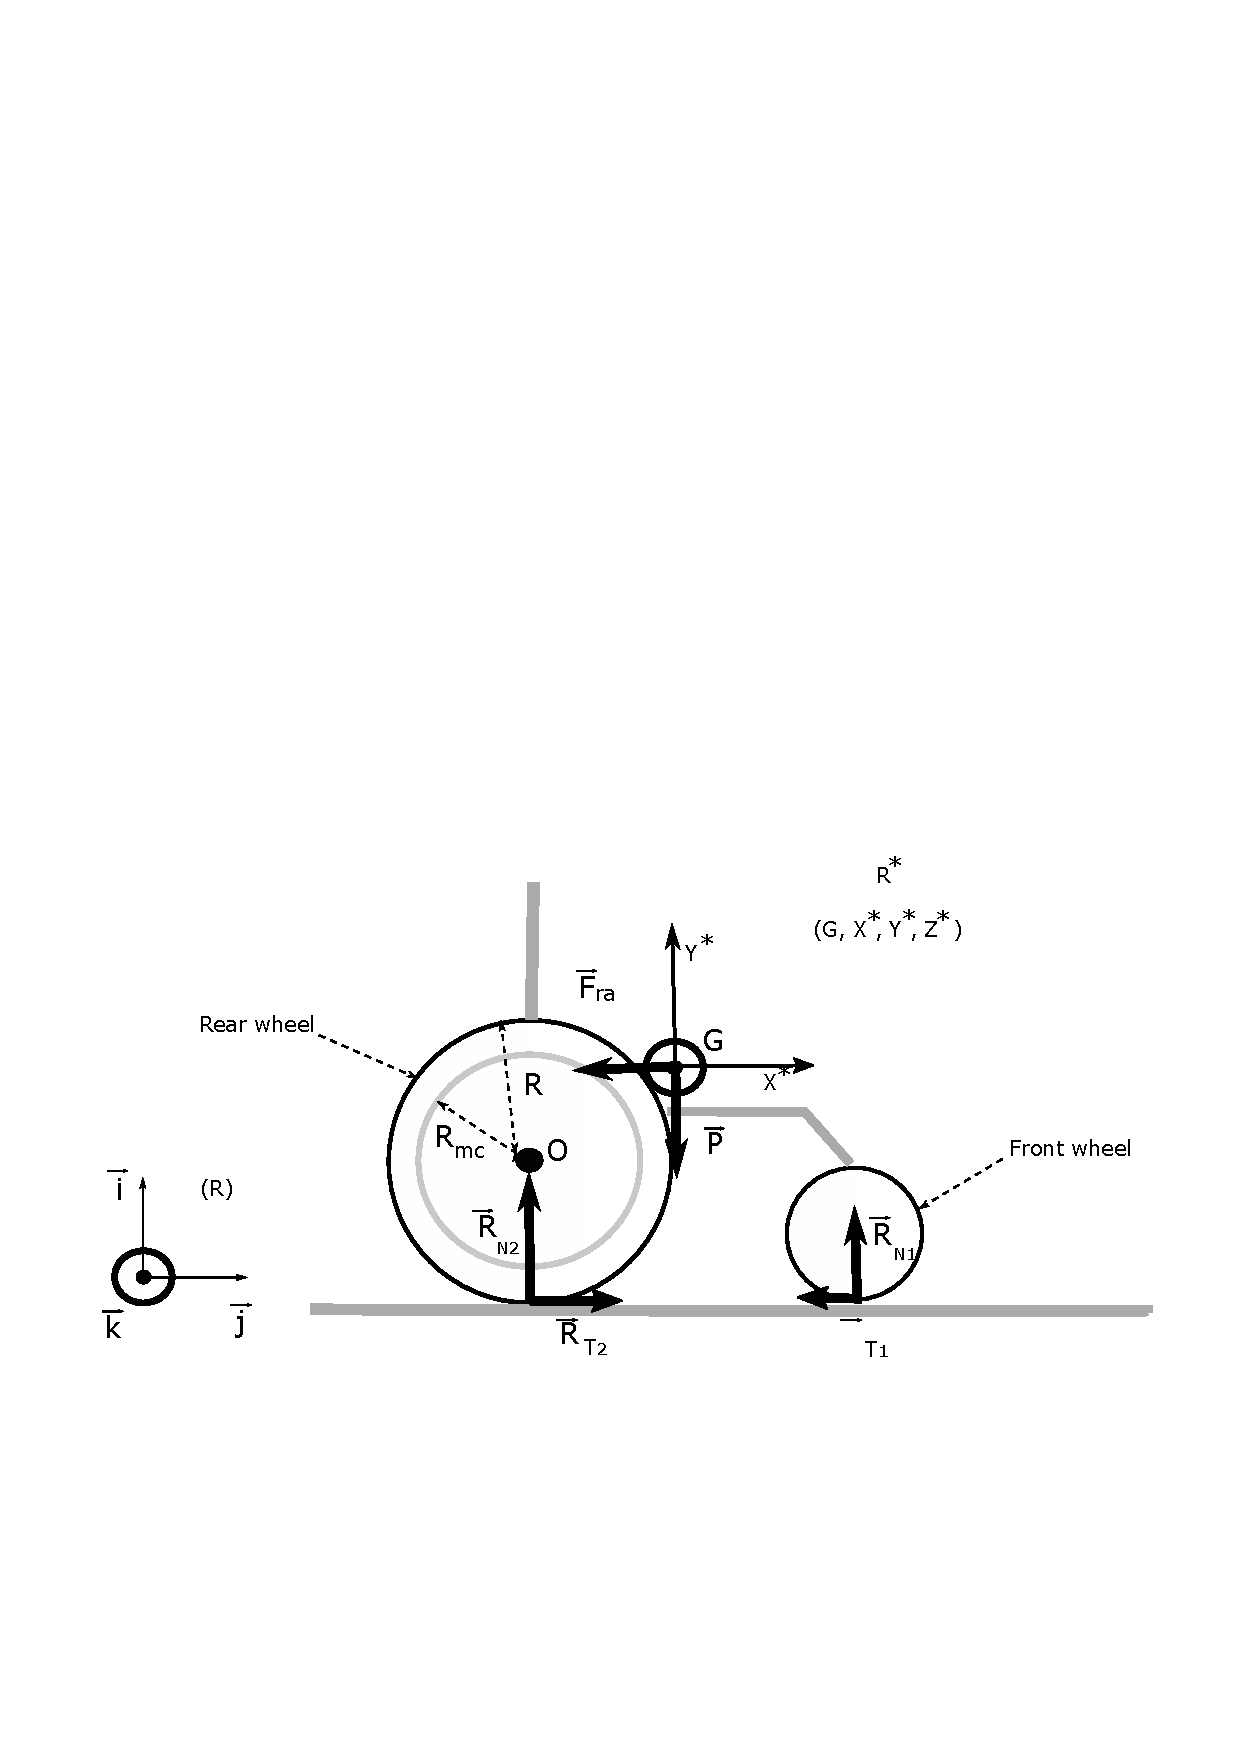
\includegraphics[scale = 0.7]{images/wheelchairModel}
\caption{Balance of forces applied to a manual wheelchair during its use; the analysis of the movement of the subject-chair system has been reduced to that of its center of gravity }
\label{Wheelchair_model}
\end{figure}

\item The doctoral thesis of Christophe SAURET (2010) [2] who proposed a method of calculating the mechanical power developed by manual wheelchair users to move. This model analyzes the kinetics (trajectory and speed) of the subject segments and the Manual Wheelchair. A segment is the body part of a user or a manual wheelchair between two markers. Figure 1.2 shows the layout of the markers used for this analysis.

\begin{figure}[h]
\center
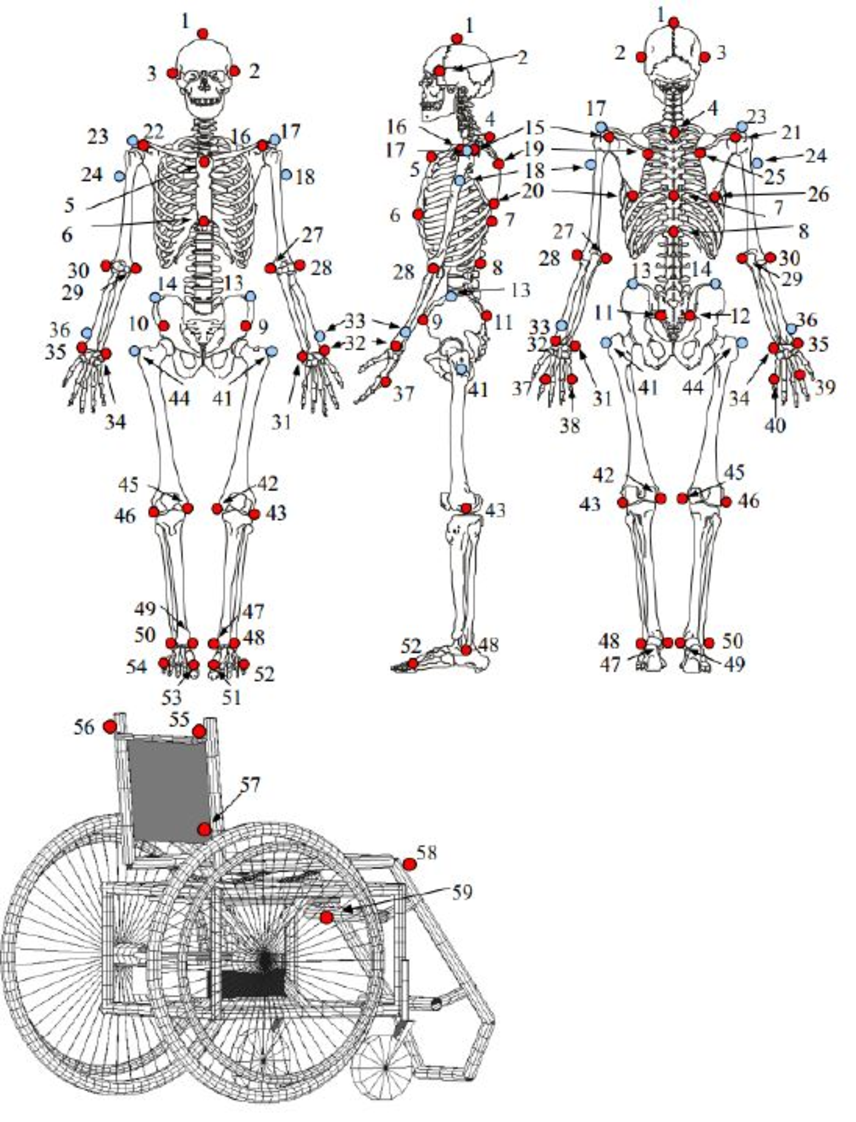
\includegraphics[scale = 0.7]{images/squelette}
\caption{Balance of forces applied to a manual wheelchair during its use; the analysis of the movement of the subject-chair system has been reduced to that of its center of gravity }
\label{Wheelchair_model}
\end{figure}

\end{itemize}



\section{Conclusion}









\chapter{Clustering of time series}

\section{Introduction}
The field of computer science dealing with the extraction of time series knowledge is known as Temporal Knowledge Discovery  which aims to extract from the knowledge of time series. But, what is a time series?

There are four categories of data concerning temporality [4]:
\begin{itemize}
\item Static data: these are data with no context
temporal we have for example the radius of a wheel, the circumference of a circle, the gravity in a place.
\item Sequences: This is an ordered sequence of events. This category includes an order but not time. As an example, we can cite a DNA sequence (GTTTTCCCAGTCACGAC) [5].
\item Time-indexed data: this is a temporal sequence of data; for example a set of measures taken at a more or less regular time interval.
\item Full-time data: Each tuple has one or more time components. In this work, we refer to time series of indexed data by the time.
\end{itemize}


Time series analysis has two main and non-disjoint objectives which are:

\begin{itemize}
\item The prediction of missing values of a time series [6].
\item The evaluation of dissimilarity or the classification of time series.
\end{itemize}

Althoug prediction is an important task of temporal data mining, the classification of time series remains its main challenge. In fact, in many cases, the prediction of missing values of time series is based on the study of time series that are similar to it, i.e., that belong to the same class as the latter [4]


Han and Kamber [1] classified clustering methods developed for handing various static data into five major categories: partitioning methods, hierarchical methods, density based methods,  grid-based  methods,  and  model-based  methods. Three of the five major categories of clustering methods for static data, specifically partitioning methods, hierarchical methods,  and  model  based  methods,  have  been  utilized directly or modified for time series clustering.

Two key aspects for achieving effectiveness and efficiency when managing time series data are representation methods and similarity measures. Time series are essentially high dimensional data and directly dealing with such data in its raw format is very expensive in terms of processing and storage cost. It is thus highly desirable to develop representation techniques that can reduce the dimensionality of time series, while still preserving the fundamental characteristics of a particular data set. Many techniques have been proposed in
 
the literature for representing time series with reduced dimensionality [2], such as Discrete Fourier Transformation, Single  Value  Decomposition,  Discrete  Cosine Transformation, Discrete Wavelet Transformation, Piecewise Aggregate Approximation, Adaptive Piecewise Constant Approximation, Chebyshev polynomials, Symbolic Aggregate approximation,  Indexable  Piecewise  Linear  Approximation etc.

In conjunction with this, there are over a dozen distance measures [2] for similarity of time series data in the literature, e.g.,   Euclidean   distance   (ED),   Dynamic   Time   Warping (DTW), distance based on Longest Common Subsequence (LCSS)  ,Edit  Distance  with  Real  Penalty  (ERP)  ,  Edit Distance on Real sequence (EDR) , DISSIM , Sequence Weighted Alignment model (Swale) , Spatial Assembling Distance (SpADe)  and similarity search based on Threshold Queries (TQuEST) . Moreover, there must be some criteria on the basis of which the performance of time series clustering method must be evaluated. Two different categories of evaluation are given based on known ground truth and unknown ground truth [3].

The rest of this paper is organized as follows: Section 2 explains Major time series approaches in three subsections. Subsection 2.1 explains Taxonomy-based-approaches. In subsections 2.2 and 2.3 Representations-based and Model- based approaches are explained respectively. Section 3 concludes this paper.

\section{MAJOR TIME SERIES CLUSTERING APPROACHES}

Time series clustering methods have been divided into three
major categories depending upon whether they work directly with raw data, indirectly with features extracted from the raw data, or indirectly with models built from the raw data.

\subsection{ Literature    Survey    of    Temporal- Proximity-Based Clustering Approach }
This approach usually works directly with  raw time  series data,  thus  called  raw-data-based  approach,  and  the  major
modification lies in replacing the distance/similarity measure
for static data with an appropriate one for time series.

M. Kumar [25] proposed a distance function based on the assumed independent Gaussian models of data errors and used a   hierarchical   clustering   method   to   group   seasonality sequences into a desirable number of clusters. The experimental results based on simulated data and retail data showed that the new method outperformed both k-means and Ward’s method that do not consider data errors in terms of (arithmetic) average estimation error. They assumed that data used have been preprocessed to remove the effects of non-seasonal factors and normalized to enable comparison of sales of different items on the same scale.

T.W. Liao [26] developed a two-step procedure for clustering multivariate time series of equal or unequal length. The first step   applies   the   k-means   or   fuzzy   c-means   clustering algorithm   to   time   stripped   data   in   order   to   convert multivariate real-valued time series into univariate discrete- valued time series. The converted variable is interpreted as state variable process. The second step employs the k-means or FCM algorithm again to group the converted univariate time series, expressed as transition probability matrices, into a number of clusters. The traditional Euclidean distance is used in the first step, whereas various distance measures including the symmetric version of Kullback–Liebler distance are employed in the second step.

T.W.   Liao   [27]   applied   several   clustering   algorithms including K-means, fuzzy c-means, and genetic clustering to multivariate  battle  simulation  time  series  data  of  unequal length with the objective to form a discrete number of battle states. The original time series data were not evenly sampled and made uniform by using the simple linear interpolation method.

C. S. Möller-Level  [28] , in their study of DNA Microarray data, proposed short time series (ST S) distance to measure the similarity in shape formed by the relative change of amplitude and the corresponding temporal information of uneven sampling intervals. All series are considered sampled at the same time points. By incorporating the STS distance into the standard fuzzy c-means algorithm, they revised the equations for computing the membership matrix and the prototypes (or cluster centers), thus developed a fuzzy time series clustering algorithm.

Shumway [29] proposed the clustering of nonstationary time series by applying locally stationary versions of Kullback– Leibler discrimination information measures that give optimal time–frequency statistics for measuring the discrepancy between two non-stationary time series. To distinguish earthquakes from explosions, an  agglomerative hierarchical cluster analysis was performed until a final set of two clusters was obtained.

Vit Niennattrakul and Chotirat Ann Ratanamahatana for the clustering of multimedia time series [5] applied K-means and K- medoids algorithms with dynamic time warping and demonstrated that K-means is much more generic clustering method when Euclidean distance is used, but it failed to give correct results when dynamic time warping is used as distance measure in averaging the shape of the time series. As the results   of   their   experiments,   they   have   confirmed   that dynamic time warping should not be used as subroutine with K-means   algorithm   and   K-medoids   with   dynamic   time warping gives satisfactory results.

For clustering time series gene expression data Pooya Sobhe Bidari [6] presented two phase functional clustering as a new approach in gene clustering. The proposed approach is based on finding functional patterns of time series using Fuzzy C- Means and K-means algorithms.
 
Pearson correlation similarity measure is used to extract the expression patterns of genes. In this approach, genes are clustered by K-means and FCM methods according to theirs time series expression, then patterns of gene behavior are extracted. Then, new features are defined for the genes and by calculating Pearson correlation between new feature vectors, genes with similar expression behavior are obtained which can lead to find interconnections between genes.

For detecting climate change in multivariate data Hardy Kremer [7] proposes novel clustering and clustering tracing techniques. In this novel clustering approach, time series is split  into  disjoint,  equal  length  intervals  and  then  density based   subsequence   clustering   approach   is   applied,   and dynamic time warping is used as a distance measure.

Jian Yin [9] proposed a clustering algorithm for time series data. He proposed a encoded-bitmap-approach-based swap is used  to  improve  the  classical  hierarchical  method.  Traffic flow data is used as time series and grey relation is used a similarity measure. After getting K clusters, encoded-bitmap- approach based swap is used to refine the K clusters and get the new K clusters. Experiments show that the proposed method has a better performance on the change trend of time series than classic algorithm.

Ville Hautamaki and Pekka Nykanen [10] defined an optimal prototype as an optimization problem and proposed a local search solution to it. They applied two Euclidean space clustering methods to time-series clustering: random swap and hierarchical clustering followed by k-means fine-tuning and it provided 10-22% improvements to k-medoids.

S.  Chandrakala  and  C.  Chandra  Sekhar  [11]  proposed  a density based method for clustering of multivariate time series of variable length in kernel feature space.  Kernal DBSCAN algorithm with Euclidean distance measure is used. They presented heuristic methods to find the initial values of the parameters used in our proposed algorithm. The performance of the proposed method is compared with the spectral clustering and kernel k-means clustering methods. Besides handling outliers, the proposed method performs as well as the spectral clustering method and outperforms the kernel k- means clustering method.

Dacheng Nie [13] analyzed time series by using NLCS (Normalized Longest Common Subsequence). NLCS is a similarity measurement widely used in comparing character sequences.  In  this  paper,  he  developed  the  NLCS  and presented   a   novel   algorithm   to   precisely   calculate   the similarity of time series. The algorithm used the sum of all common  subsequence  instead  of  longest  common subsequence which can’t represent the similarity of sequences accurately. The experiments based on synthetic and real-life datasets showed that the proposed algorithm performed better in comparing the similarity of time series. Comparing with Euclidean distance on four cluster validity indices, the results lead to a better performance by k-means or self-organize map. 


% Please add the following required packages to your document preamble:
% \usepackage[normalem]{ulem}
% \useunder{\uline}{\ul}{}
\begin{table}[ht]
\centering
\caption{My caption}
\label{my-label0}
\begin{tabular}{|l|l|l|l|}
\hline
\multicolumn{1}{|c|}{\textbf{Paper}}                           & \multicolumn{1}{c|}{\textbf{Distance Measure}}                                                                                               & \multicolumn{1}{c|}{\textbf{Algorithm}}                                                  & \multicolumn{1}{c|}{\textbf{Application}}                                                       \\ \hline
M. Kumar                                                       & \begin{tabular}[c]{@{}l@{}}Based      on      the      assumed\\   independent\\    \\   Gaussian models\\   of\\   data errors\end{tabular} & Agglomerative Hierarchical                                                               & Seasonality pattern in retails                                                                  \\ \hline
T.-W. Liao                                                     & \begin{tabular}[c]{@{}l@{}}Euclidean      and    \\    symmetric\\   version    of    Kullback–Liebler\\   distance\end{tabular}             & \begin{tabular}[c]{@{}l@{}}K-Means\\   and Fuzzy C-Means\end{tabular}                    & Battle simulations                                                                              \\ \hline
T.-W. Liao                                                     & Dynamic Time Warping                                                                                                                         & \begin{tabular}[c]{@{}l@{}}K-Medoids    Based  \\    Genetic\\   Clustering\end{tabular} & Battle simulations                                                                              \\ \hline
C.S. Möller-Levet                                              & \begin{tabular}[c]{@{}l@{}}Short     time     series     (STS)\\   distance\end{tabular}                                                     & Modified Fuzzy C-Means                                                                   & DNA microarray                                                                                  \\ \hline
Shumway                                                        & \begin{tabular}[c]{@{}l@{}}Kullback–Leibler\\   discrimination         information measure\end{tabular}                                      & Agglomerative Hierarchical                                                               & \begin{tabular}[c]{@{}l@{}}Earthquakes   \\    and   \\    mining\\   explosions\end{tabular}   \\ \hline
Vit Niennattrakul                                              & Dynamic Time Warping                                                                                                                         & K-Means, K-Medoids                                                                       & \begin{tabular}[c]{@{}l@{}}Multimedia time\\   series\end{tabular}                              \\ \hline
\begin{tabular}[c]{@{}l@{}}Pooya Sobhe\\   Bidari\end{tabular} & Pearson Correlation                                                                                                                          & K-Means, Fuzzy C-Means                                                                   & Pattern extraction in genes                                                                     \\ \hline
Hardy Kremer                                                   & Dynamic Time Warping                                                                                                                         & \begin{tabular}[c]{@{}l@{}}Density   Based \\    Subsequence\\   Clustering\end{tabular} & \begin{tabular}[c]{@{}l@{}}Detecting climate\\   change\end{tabular}                            \\ \hline
Jian Yin                                                       & Grey Relation                                                                                                                                & Hierarchical Clustering                                                                  & \begin{tabular}[c]{@{}l@{}}Change\\    trend  of\\    traffic  flow\\   data\end{tabular}       \\ \hline
S. Chandrakala                                                 & Euclidean                                                                                                                                    & Kernal DBScan                                                                            & \begin{tabular}[c]{@{}l@{}}Multivariate       time     \\    series\\   clustering\end{tabular} \\ \hline
Aurangzeb Khan                                                 & Euclidean                                                                                                                                    & \begin{tabular}[c]{@{}l@{}}K-Mean+ MFP(Most Frequent\\   Pattern)\end{tabular}           & Stock and inventory data                                                                        \\ \hline
Mengfan Zhang                                                  & \begin{tabular}[c]{@{}l@{}}CVT(Computational          Verb\\   Theory)\end{tabular}                                                          & K-Means                                                                                  & Stock market data                                                                               \\ \hline
S.R.Nanda                                                      & Euclidean                                                                                                                                    & K-Means                                                                                  & Portfolio management                                                                            \\ \hline
Jianfei Wu                                                     & N/A                                                                                                                                          & K-Means                                                                                  & Stock data                                                                                      \\ \hline
\end{tabular}
\end{table}


Aurangzeb  Khan  [16]  used  hybrid  clustering  algorithm  to mine the frequent pattern in the stock or inventory data. He proposed an algorithm for mining patterns of huge stock data to predict factors affecting the sale of products. In the first phase of his method, he applied k-means algorithm to divide the stock data into  three different clusters i.e. Dead Stock (DS), Slow Moving (SM) and Fast Moving (FM) on the basis of product categories. In the second phase, he applied Most Frequent Pattern (MFP) algorithm to find frequencies of property values  of the  corresponding items. MFP  provides frequent  patterns  of  item  attributes  in  each  category  of products and also gives sales trend in a compact form. The experimental result showed that the proposed hybrid k-mean plus MFP algorithm can generate more useful pattern from large stock.

Songpol Ongwattanakul [15] and Dararat Srisai introduced a new variation of Dynamic time warping distance measure for time series shape averaging classification. According to them resampled DTW and Hybrid DTW give better accuracy and
 
high  performance  than  original  DTW  but  to  improve  the
accuracy further they introduced Contrast Enhanced Dynamic
Time Warping (CEDTW) that reduces the effect from data points  that  have  non-trivial  contribution  to  the  measured
distance and improves the accuracy in similarity measure.

Xueyan WU [17] proposed a method of data stream clustering for stock data analysis. The method aimed to retain shape and tend features during the clustering process. He divided the process of the proposed method into two parts i.e. online clustering and offline macro clustering. Online clustering extracted   data   flow   characteristics   and   maintains   the clustering feature vectors and offline macro clustering is the process which responded to user requests and achieved clustering. Experiments showed that the method had good results.

Aurangzeb  Khan  [16]  used  hybrid  clustering  algorithm  to mine the frequent pattern in the stock or inventory data. He proposed an algorithm for mining patterns of huge stock data to predict factors affecting the sale of products. In the first phase of his method, he applied k-means algorithm to divide the stock data into  three different clusters i.e. Dead Stock (DS), Slow Moving (SM) and Fast Moving (FM) on the basis of product categories. In the second phase, he applied Most Frequent Pattern (MFP) algorithm to find frequencies of property values  of the  corresponding items. MFP  provides frequent  patterns  of  item  attributes  in  each  category  of products and also gives sales trend in a compact form. The experimental result showed that the proposed hybrid k-mean plus MFP algorithm can generate more useful pattern from large stock.

Xueyan WU [17] proposed a method of data stream clustering for stock data analysis. The method aimed to retain shape and tend features during the clustering process. He divided the process of the proposed method into two parts i.e. online clustering and offline macro clustering. Online clustering extracted   data   flow   characteristics   and   maintains   the clustering feature vectors and offline macro clustering is the process which responded to to user requests and achieved clustering. Experiments showed that the method had good results.

Mengfan Zhang [18] and Tao Yang applied the computational verb theory (CVT) to analyze the stock market data. His goal was to find the most representative trends in the intra-day stock   market   data.   First   round   of   computational   verb clustering algorithm was used to categorize the stock market data and in the second round of computational verb k-means clustering algorithm is used to refine the representative trends in the stock market data. Experiments showed that the applied method yielded the most representative curves in the stock market data.

Jianfei Wu [19] introduced an algorithm that used stock sector information directly in conjunction with time series subsequences for mining core patterns within the sectors of stock market data. He used the stream sliding window concepts. Two adjacent sliding windows were used, namely training window and evaluation window. The algorithm detected significant sectors in the training window, and built core patterns for the significant ones. The algorithm identified whether a stock sector currently shows coherent behavior. When coherent behavior of a stock sector was detected, core patterns were extracted. The core patterns were more stable than  clusters found by some clustering algorithm DBScan. Through comparing with DBScan, we show the effectiveness of the proposed algorithm.

Huawang Shi [20] proposed a novel unascertained C-means clustering algorithm. He used the theory and method of unascertained measure and established clustering weights and a novel unascertained C-means clustering algorithm. Experimental results showed that the proposed method performed  more  robust  to  noise  than  the  fuzzy  C-means (FCM) clustering algorithm do.

S.R.Nanda [23] applied clustering to stock market data for portfolio  management.  She  used  stock  returns  at  different times along with their valuation ratios and results analysis showed that k-means cluster analysis builds the most compact cluster as compared to SOM and Fuzzy C-means for stock classification data. She then selected stocks from clusters to build portfolio, minimizing portfolio risk and compared the returns with that of benchmark index.
 
\subsection{ Literature Survey of Representation- Based Clustering Approach}
It is not easy to work directly with the raw data that are highly noisy. Feature based approach first converts a raw time series data  into  a  feature  vector  of  lower  dimension  and  then
clustering algorithms are applied.

T.-C. Fu [30] described the use of self-organizing maps for grouping data sequences segmented from the numerical time series  using  a  continuous  sliding  window  with  the  aim to discover similar temporal patterns dispersed along the time series. They introduced the perceptually important point (PIP) identification algorithm to reduce the dimension of the input data sequence in accordance with the query sequence. The distance measure between the PIPs found was defined as the sum of the mean squared distance along the vertical scale (the magnitude) and that along the horizontal scale (time dimension). To process multi resolution patterns, training patterns from different resolutions are grouped into a set of training samples to which the SOM clustering process is applied  only  once.  Two  enhancements  were  made  to  the SOM: filtering out those nodes (patterns) in the output layer that did not participate in the recall process and consolidating the discovered patterns with a relatively more general pattern by a redundancy removal step.

Dong Jixue [8] for mining the financial time series uses the wave cluster, which is a kind of grid cluster and the density cluster unify. In this, basic details and methods of phase space reconstruction are analyzed in details. All of these provided the theoretical basis and technical feasibility to time series data mining based on phase space reconstruction. After contrasting the different means of time series pattern mining, the problem of Time Series Data Mining framework TSDM is pointed out, and the temporal patterns mining method based Wave cluster is systematically presented. By the multiresolution property of wavelet transformations and the grid-based  partition  method, it could  detect arbitrary-shape clusters at different scales and levels of detail.

Huiting Liu [12] proposed  a new similar pattern  matching method.  Firstly,  trends  of  time  series  are  extracted  by empirical mode decomposition, and the trends are translated into vectors to realize dimension reduction. Secondly, the vectors are clustered by a forward propagation learning algorithm. Finally, all the series that is similar with the query are found by calculating Euclidean distance between the query and the series that belong to the same category with it. Experimental results showed that EMD outperforms the FFT (Fast Fourier Transform) when they are used to reduce dimension. 


\begin{table}[ht]
\centering
\caption{My caption}
\label{my-label1}
\begin{tabular}{|l|l|l|l|l|}
\hline
\multicolumn{1}{|c|}{\textbf{Paper}} & \multicolumn{1}{c|}{\textbf{Features}}                                     & \multicolumn{1}{c|}{\textbf{\begin{tabular}[c]{@{}c@{}}Distance\\   Measure\end{tabular}}}                                    & \multicolumn{1}{c|}{\textbf{Clustering Algorithm}}                                 & \multicolumn{1}{c|}{\textbf{Application}}                                              \\ \hline
T.-C. Fu                             & \begin{tabular}[c]{@{}l@{}}Perceptually important\\   points\end{tabular}  & \begin{tabular}[c]{@{}l@{}}Sum of the mean\\   squared distance along the\\   vertical and horizontal\\   scales\end{tabular} & Modified SOM                                                                       & Hong Kong stock market                                                                 \\ \hline
M. Vlachos                           & \begin{tabular}[c]{@{}l@{}}Haar wavelet\\   transform\end{tabular}         & Euclidean                                                                                                                     & Modified k-means                                                                   & Non-specific                                                                           \\ \hline
Huiting Liu                          & \begin{tabular}[c]{@{}l@{}}Empirical mode\\   decomposition\end{tabular}   & Euclidean                                                                                                                     & \begin{tabular}[c]{@{}l@{}}Forward propagation\\   learning algorithm\end{tabular} & Non-specific                                                                           \\ \hline
Chonghui GUO                         & \begin{tabular}[c]{@{}l@{}}Independent component\\   analysis\end{tabular} & Euclidean                                                                                                                     & Modified k-means                                                                   & \begin{tabular}[c]{@{}l@{}}Real world stock time-\\   series\end{tabular}              \\ \hline
Jian Xin Wu                          & \begin{tabular}[c]{@{}l@{}}Independent component\\   analysis\end{tabular} & N/A                                                                                                                           & \begin{tabular}[c]{@{}l@{}}support vector\\   regression\end{tabular}              & Financial time-series                                                                  \\ \hline
Geert Verdoolaege                    & Wavelet transform                                                          & \begin{tabular}[c]{@{}l@{}}Kullback- Liebler\\   divergence\end{tabular}                                                      & k-means                                                                            & \begin{tabular}[c]{@{}l@{}}Detection of activated\\   voxels in FMRI data\end{tabular} \\ \hline
Liu Suyi                             & Hough transform                                                            & N/A                                                                                                                           & Mean shift algorithm                                                               & \begin{tabular}[c]{@{}l@{}}Feature recognition of\\   underwater images\end{tabular}   \\ \hline
Dong Jixue                           & Wavelet transform                                                          & N/A                                                                                                                           & \begin{tabular}[c]{@{}l@{}}Grid-based partitioning\\   method\end{tabular}         & Financial time-series                                                                  \\ \hline
\end{tabular}
\end{table}


M.   Vlachos   [31]   presented   an   approach   to   perform incremental clustering of time series at  various resolutions using the Haar wavelet transform. First, the Haar wavelet decomposition is computed for all-time series. Then, the k- means clustering algorithm is applied, starting at the coarse level  and  gradually  progressing  to  finer  levels.  The  final centers at the end of each resolution are reused as the initial centers for the next level of resolution. Since the length of the data reconstructed from the Haar decomposition doubles as we progress to the next level, each coordinate of the centers at the end of level i is doubled to match the dimensionality of the points on level i+1. The clustering error is computed at the end  of  each  level  as  the  sum  of  number  of  incorrectly clustered objects for each cluster divided by the cardinality of the dataset.

Nicole Powell [14] compared unsupervised classification techniques such as k-means clustering with supervised classification techniques such as support vector machines for stock   prices   forecasting   .He   used   Principal   component analysis to reduce the dimension of the data set to select the component which have the biggest effect and concluded that for this application both method give comparable results but unsupervised  classification  techniques  are  better  for  stock trend forecasting because unsupervised methods fine pattern in data that is usually seen as uncorrelated.

Anthony J. T .Lee [24] presented an effective approach (Hierarchical agglomerative and recursive k-means clustering) to stock market prediction. The proposed method converted each financial report to feature vector and used hierarchical agglomerative  clustering  to  divide  this  feature  vector  into
 
clusters and then, for each sub-cluster so that most feature vectors in each sub-clusters belonged to the same class. Then, for each sub-cluster, a centroid was chosen as the representative feature vector and finally this feature vector was employed to predict the stock price movements.

Chonghui GUO [22] presented a novel feature based approach to time series clustering which first converted the raw time series into feature vector of lower dimension by using ICA (Independent  Component  Analysis)     algorithm  and  then applied a modified k-means clustering algorithm to the extracted feature vector . Finally to validate the feasibility and effectiveness of the proposed approach he used it to analyze the real world stock time series and achieved the reasonable results.

Jian   Xin   Wu   [32]   proposed   a   combination   of   ICA (independent component analysis) with SVR (support vector regression) for predicting the financial time series. The proposed method used SRM (structure risk minimization) principle.  It  removed  the  problem  of  learning  algorithms based on ERM (empirical risk minimization) principle, which always have good fit for the training samples, but bad prediction for future samples. He used non-linear SVR (Support vector regression) for the prediction, and before applying SVR, he used ICA for the feature extraction. ICA considers independence which is a more strict condition than PCA which takes into account uncorrelated between features.

Geert Verdoolaege [33] proposed a new method for the detection of activated voxels in event related BOLD FMRI data. Firstly, he derived wavelet histograms from each voxel time series and modeled the derived statistics through GGD (generalized Gaussian distribution). Finally, he performed the K-Means clustering of the GGD’s characterizing the voxel data in a synthetic data set using the KLD (Kullback- Liebler divergence) as a similarity measure.

The main issue of similarity search in time series database is to improve the search performance since time series data is usually  is  of  high  dimension  and  for  this  is  important  to reduce the search space for the efficient processing of similarity search. In this paper, D.Muruga Radha Devi [34], proposed  a  combination  of  using  Vari-DWT  and  Polar wavelet. Vari-DWT is fast to compute and requires little storage for each sequence; it preserves Euclidean distance and allows good approximation with a subset of coefficients. But its drawbacks are, it shows poor performance for locally distributed time series data since it uses averages to reduce the dimensionality of the data and another limitation is it works
best when the length of the time series is 2n, and hence becomes the reason of using Polar wavelet, it uses polar co-
ordinates which are not affected from averages and, it works with the time sequences of any length without distorting the original   signal.   She   evaluated   the   effectiveness   of  this approach by using real weather data and synthetic datasets.

Liu Suyi [35] did feature recognition for underwater images. Firstly, the preprocessing of underwater image was done to improve image quality so that seam feature could be recognized easily. Weld featured image was effectively segmented by Mean Shift Algorithm, and finally Hough Transform was used to recognize the feature of underwater weld images.

\subsection{Literature Survey of Model-Based}
Clustering Approach
This class of approaches considers that each time series is
generated by some kind of model or probability distributions. Time series are considered similar when the models characterizing  individual  series  or  the  remaining  residuals after fitting the model are similar.

Baragona [36] evaluated three meta-heuristic methods for partitioning a set of time series into clusters in such a way that (i)  the  cross-correlation  maximum  absolute  value  between each pair of time series that belong to the same cluster is greater than some given threshold, and (ii) the k-min cluster criterion is minimized with a specified number of clusters. The cross-correlations are computed from the residuals of the models of the original time series. Among all methods evaluated,  Tabu  search  was  found  to  perform  better  than single linkage, pure random search, simulation annealing and genetic algorithms based on a simulation experiment on ten sets of artificial time series generated from low-order univariate and vector ARMA models.

K.  Kalpakis    [37]  studied  the  clustering  of  ARIMA  time series, by using the Euclidean distance between the Linear Predictive Coding cepstra of two time-series as their dissimilarity measure. The cepstral coefficients for an AR(p) time series are derived from the auto-regression coefficients. The partition around medoids method that is a k-medoids algorithm was chosen, with the clustering results evaluated with  the  cluster  similarity  measure  and  Silhouette  width. Based on a test of four data sets, they showed that the LPC cestrum provides higher discriminatory power to tell one time series from another and superior clustering than other widely used methods such as the Euclidean distance between (the
 
first 10 coefficients of) the DFT, DWT, PCA, and DFT of the auto-correlation function of two time series.

Xiong and Yeung [38] proposed a model-based method for clustering univariate ARIMA series. They assumed that the time series are generated by k different ARMA models, with each model corresponds to one cluster of interest. An expectation-maximization (EM) algorithm was used to learn the mixing coefficients as well as the parameters of the component models that maximize the expectation of the complete-data log-likelihood. In addition, the EM algorithm was improved so that the number of clusters could be determined automatically.

L. Wang [39] presented a framework for tool wear monitoring in a machining process using discrete hidden Markov models. The feature vectors are extracted from the vibration signals measured during turning operations by wavelet analysis. The extracted  feature vectors are then  converted into a symbol sequence  by vector  quantization,  which  in  turn  is used  as input for training the hidden Markov model by the expectation maximization approach. Yun Yang and Ke Chen [4] presented an unsupervised ensemble learning approach to time series clustering by combining RPCL (rival-penalized competitive learning) with different representations. This approach first exploits its capability of RPCL rule in clustering analysis of automated model selection on individual representations and then applies ensemble learning for the synergy of reconciling diverse partitions resulted from the use of different representations and augmenting RPCL network in automatic model selection and overcoming its inherent limitation. They evaluated their approach on 16 benchmark time series data mining task. Simulation results demonstrated that their approach yielded favorite results in clustering analysis of automatic model selection.

Yu-Chia Hsu [4] proposed a approach using self organizing map (SOM) for time series data clustering and similar pattern recognition to improve the optimal hedge ratio (OHR) estimation. Taiwan stock market hedging is used. Five SOM based models and two traditional models were compared in this approach. Experiments demonstrated the SOM approach provides a useful alternative to the OHR estimation.

Xin Huang proposed [40] a research on predicting agriculture drought based on fuzzy set and R/S analysis model. He used fuzzy clustering iteration method to cluster the data of many years rainfall and then considered sensitiveness coefficient as the foundation of calculating weight, which affected the crop output by valid rainfall in each growth stage. The results of application showed that the model is convenient and feasible in the application of forecasting the years of occurrence in agriculture drought.

Yupei Lin [41] tried to improve the prediction accuracy with correcting two deficiencies, sub intervals failing to well represent the data distribution structures and a single antecedent factor in the fuzzy relationship in current fuzzy time series model. First, he partitioned the universe of discourse in subintervals with the midpoints of two adjacent clusters centers, and the subintervals are employed to fuzzify the time series into fuzzy time series. Then, the fuzzy time series model with multi factors high order fuzzy relationship is built-up to forecast the stock market. The results showed that the model improved the prediction accuracy when compared with the benchmark model.

Shan Gao [42] analyzed ARCH (Autoregressive Conditional
Heteroscedasticity) effects of wind data series with Eviews 

software. Firstly, he built an ARMA (Autoregressive Moving Average)  model of wind  speed  time  series and, tested the ARCH effect of residual ARMA Model by Lagrange Multiplier. Lastly, he compared the forecasting performances of ARMA-ARCH model with ARMA model and proved that ARMA-ARCH model possesses higher accuracy.


\begin{table}[ht]
\centering
\caption{My caption}
\label{my-label2}
\begin{tabular}{|l|l|l|l|l|}
\hline
\multicolumn{1}{|c|}{\textbf{Paper}} & \multicolumn{1}{c|}{\textbf{Model}}                                                     & \multicolumn{1}{c|}{\textbf{Distance measure}}                      & \multicolumn{1}{c|}{\textbf{\begin{tabular}[c]{@{}c@{}}Clustering\\   algorithm\end{tabular}}} & \multicolumn{1}{c|}{\textbf{Application}}                                              \\ \hline
Baragona                             & ARMA                                                                                    & \begin{tabular}[c]{@{}l@{}}Cross-correlation\\   based\end{tabular} & \begin{tabular}[c]{@{}l@{}}Tabu    search,  \\    GA\\   and\end{tabular}                      & Non-specific                                                                           \\ \hline
K. Kalpakis                          & AR                                                                                      & Euclidean                                                           & Partitioning   around medoids                                                                  & Public data                                                                            \\ \hline
Xiong and Yeung                      & ARMA mixture                                                                            & Log-liklihood                                                       & EM learning                                                                                    & Public data                                                                            \\ \hline
L. Wang                              & Discrete HMM                                                                            & Log-liklihood                                                       & EM learning                                                                                    & \begin{tabular}[c]{@{}l@{}}Tool        \\    condition\\   monitoring\end{tabular}     \\ \hline
Xin Huang                            & \begin{tabular}[c]{@{}l@{}}Fuzzy  set\\    and\\    R/S\\   analysis model\end{tabular} & N/A                                                                 & \begin{tabular}[c]{@{}l@{}}Fuzzy     \\    clustering iteration method\end{tabular}            & \begin{tabular}[c]{@{}l@{}}Predicting\\   agriculture drought\end{tabular}             \\ \hline
Shan Gao                             & ARMA-ARCH                                                                               & N/A                                                                 & N/A                                                                                            & \begin{tabular}[c]{@{}l@{}}To analyze the\\   effects of wind data series\end{tabular} \\ \hline
\end{tabular}
\end{table}

\section{CONCLUSIONS}
In recent years, there has been variety of interests in mining time series. Particularly, the clustering of time series has attracted the interest of researchers. As Time series data are frequently large and may contain outliers, therefore careful
examination of the proposed algorithms is necessary. In this paper we have studied most recent techniques on the subject of time series clustering. The uniqueness and limitation of previous research are discussed and several possible topics for future research are identified. It is hoped that this review will
serve as the steppingstone for those interested in advancing this area of research.

